\documentclass{standalone}
\usepackage{libertinus}
\usepackage{tikz}
\usetikzlibrary{matrix, patterns, backgrounds, positioning}
\begin{document}
	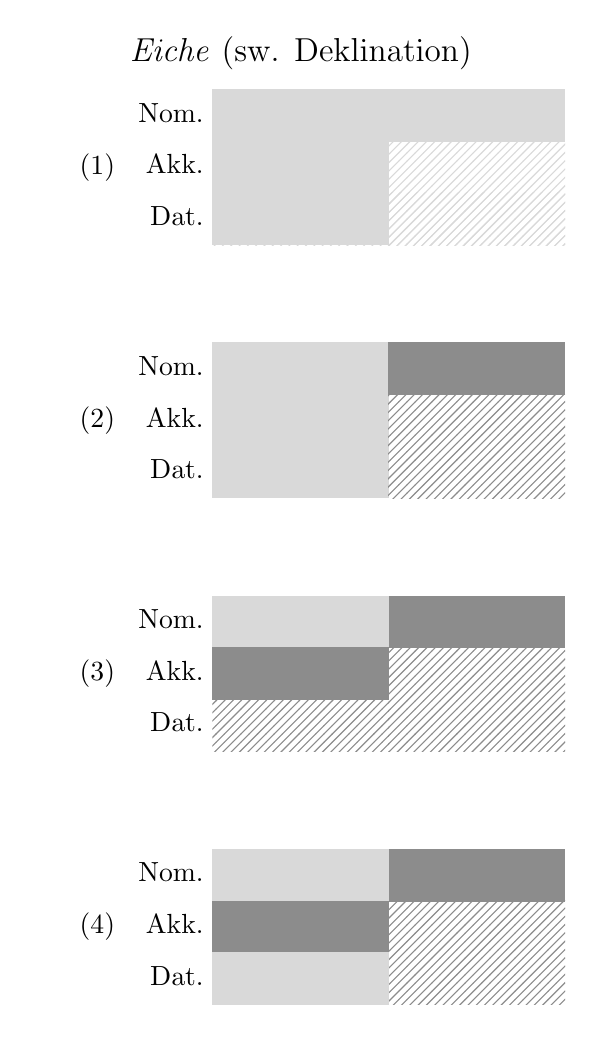
\begin{tikzpicture}
		\matrix [matrix of nodes,
		nodes in empty cells,
		align=right,
		nodes={text width=2cm, minimum height=1em, font=\strut}]
		(eiche1)
		{
			Nom.& & \\
			Akk.& & \\
			Dat.& & \\
		};
		\fill [fill=gray!30] 
		(eiche1-1-2.north west) rectangle (eiche1-3-2.south east);
		\fill [fill=gray!30]
		(eiche1-1-3.north west) rectangle (eiche1-1-3.south east);
		\fill [pattern=north east lines, pattern color=gray!30]
		(eiche1-2-3.north west) rectangle (eiche1-3-3.south east);
		\fill[pattern=north east lines, pattern color=gray!30]
		(eiche1-3-2.north west) rectangle (eiche1-3-3.south east);
		\node[left = 0cm of eiche1-2-1.center] {(1)};
		\node[font=\large,anchor=south] at (eiche1.north) {\textit{Eiche} (sw. Deklination)};
		
		\matrix [matrix of nodes,
		nodes in empty cells,
		align=right,
		below = of eiche1,
		nodes={text width=2cm, minimum height=1em, font=\strut}]
		(eiche2)
		{
			Nom.& & \\
			Akk.& & \\
			Dat.& & \\
		};
		\fill [fill=gray!30] 
		(eiche2-1-2.north west) rectangle (eiche2-3-2.south east);
		\fill [fill=gray!90]
		(eiche2-1-3.north west) rectangle (eiche2-1-3.south east);
		\fill [pattern=north east lines, pattern color=gray!90]
		(eiche2-2-3.north west) rectangle (eiche2-3-3.south east);
		\node[left = 0cm of eiche2-2-1.center] {(2)};
		
		\matrix [matrix of nodes,
		nodes in empty cells,
		align=right,
		below = of eiche2,
		nodes={text width=2cm, minimum height=1em, font=\strut}]
		(eiche3)
		{
			Nom.& & \\
			Akk.& & \\
			Dat.& & \\
		};
		\node[left = 0cm of eiche3-2-1.center] {(3)};
		\fill [fill=gray!90]
		(eiche3-1-3.north west) rectangle (eiche3-1-3.south east);
		\fill [pattern=north east lines, pattern color=gray!90]
		(eiche3-2-3.north west) rectangle (eiche3-3-3.south east);
		\fill[gray!30]
		(eiche3-1-2.north west) rectangle (eiche3-1-2.south east);
		\fill[gray!90]
		(eiche3-2-2.north west) rectangle (eiche3-2-2.south east);
		\fill[pattern=north east lines, pattern color=gray!90] 
		(eiche3-3-2.north west) rectangle (eiche3-3-2.south east);
		
		\matrix [matrix of nodes,
		nodes in empty cells,
		align=right,
		below = of eiche3,
		nodes={text width=2cm, minimum height=1em, font=\strut}]
		(eiche4)
		{
			Nom.& & \\
			Akk.& & \\
			Dat.& & \\
		};
		\node[left = 0cm of eiche4-2-1.center] {(4)};
		\fill [fill=gray!90]
		(eiche4-1-3.north west) rectangle (eiche4-1-3.south east);
		\fill [pattern=north east lines, pattern color=gray!90]
		(eiche4-2-3.north west) rectangle (eiche4-3-3.south east);
		\fill[gray!30]
		(eiche4-1-2.north west) rectangle (eiche4-1-2.south east);
		\fill[gray!90]
		(eiche4-2-2.north west) rectangle (eiche4-2-2.south east);
		\fill[gray!30] 
		(eiche4-3-2.north west) rectangle (eiche4-3-2.south east);
	\end{tikzpicture}
\end{document}